\documentclass[10pt,border=1pt]{standalone}
\usepackage[T1]{fontenc}
\usepackage{mathptmx}
\usepackage{amsmath,amssymb}
\usepackage[table]{xcolor}
\usepackage{tikz}
\usetikzlibrary{positioning,arrows.meta,calc,fit,decorations.pathreplacing}
\definecolor{fmblue}{HTML}{2A78D6}
\definecolor{cnnorange}{HTML}{EB6834}
\definecolor{inkgray}{HTML}{52514E}
\definecolor{lightfill}{HTML}{F1F0EC}
\tikzset{
  arr/.style={-{Stealth[length=2.2mm]}, draw=inkgray, line width=0.7pt},
  blk/.style={draw=inkgray, rounded corners=2pt, fill=white, align=center, inner sep=3pt, font=\fontsize{10}{12}\selectfont},
  frz/.style={blk, fill=lightfill},
  trn/.style={blk, fill=fmblue!14},
  trn2/.style={blk, fill=cnnorange!16},
  note/.style={align=left, font=\fontsize{10}{12}\selectfont\itshape, text=inkgray},
}
\begin{document}
\fontsize{10}{12}\selectfont

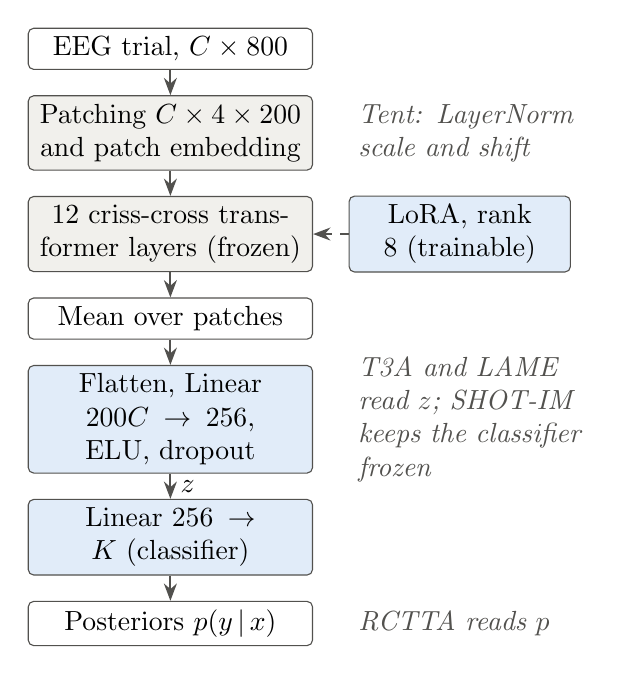
\begin{tikzpicture}[node distance=0.32cm]
\node[blk, text width=3.4cm] (x) {EEG trial, $C\times800$};
\node[frz, text width=3.4cm, below=of x] (pe) {Patching $C\times4\times200$ and patch embedding};
\node[frz, text width=3.4cm, below=of pe] (tr) {12 criss-cross transformer layers (frozen)};
\node[trn, text width=2.6cm, right=0.45cm of tr] (lo) {LoRA, rank 8 (trainable)};
\node[blk, text width=3.4cm, below=of tr] (mp) {Mean over patches};
\node[trn, text width=3.4cm, below=of mp] (h1) {Flatten, Linear $200C\to256$, ELU, dropout};
\node[trn, text width=3.4cm, below=of h1] (fc) {Linear $256\to K$ (classifier)};
\node[blk, text width=3.4cm, below=of fc] (p) {Posteriors $p(y\,|\,x)$};
\draw[arr] (x)--(pe); \draw[arr] (pe)--(tr); \draw[arr] (tr)--(mp); \draw[arr] (mp)--(h1);
\draw[arr] (h1)--node[right, font=\fontsize{10}{12}\selectfont]{$z$}(fc); \draw[arr] (fc)--(p);
\draw[arr, dashed] (lo)--(tr);
\node[note, text width=2.9cm, right=0.45cm of h1] {T3A and LAME read $z$; SHOT-IM keeps the classifier frozen};
\node[note, text width=2.9cm, right=0.45cm of pe] {Tent: LayerNorm scale and shift};
\node[note, text width=2.9cm, right=0.45cm of p] {RCTTA reads $p$};
\end{tikzpicture}
\end{document}
